\documentclass{TDP003mall}

\usepackage{graphicx}
\usepackage{float}

\newcommand{\version}{Version 1.0}
\author{Jimmie Roos, \url{jimro697@student.liu.se}\\
        Sebastian Grunditz, \url{sebgr273@student.liu.se}}
\title{LoFi-prototyp för TDP003}
\date{2018-09-20}
\rhead{Jimmie Roos\\
      Sebastian Grunditz}



\begin{document}
\projectpage
\section{Revisionshistorik}
\begin{table}[!h]
\begin{tabularx}{\linewidth}{|l|X|l|}
\hline
Ver. & Revisionsbeskrivning & Datum \\\hline
1.0 & Dokument skapat och bilder tillagda \\\hline
\end{tabularx}
\end{table}


\section{Startsida}
\begin{figure}[H]
  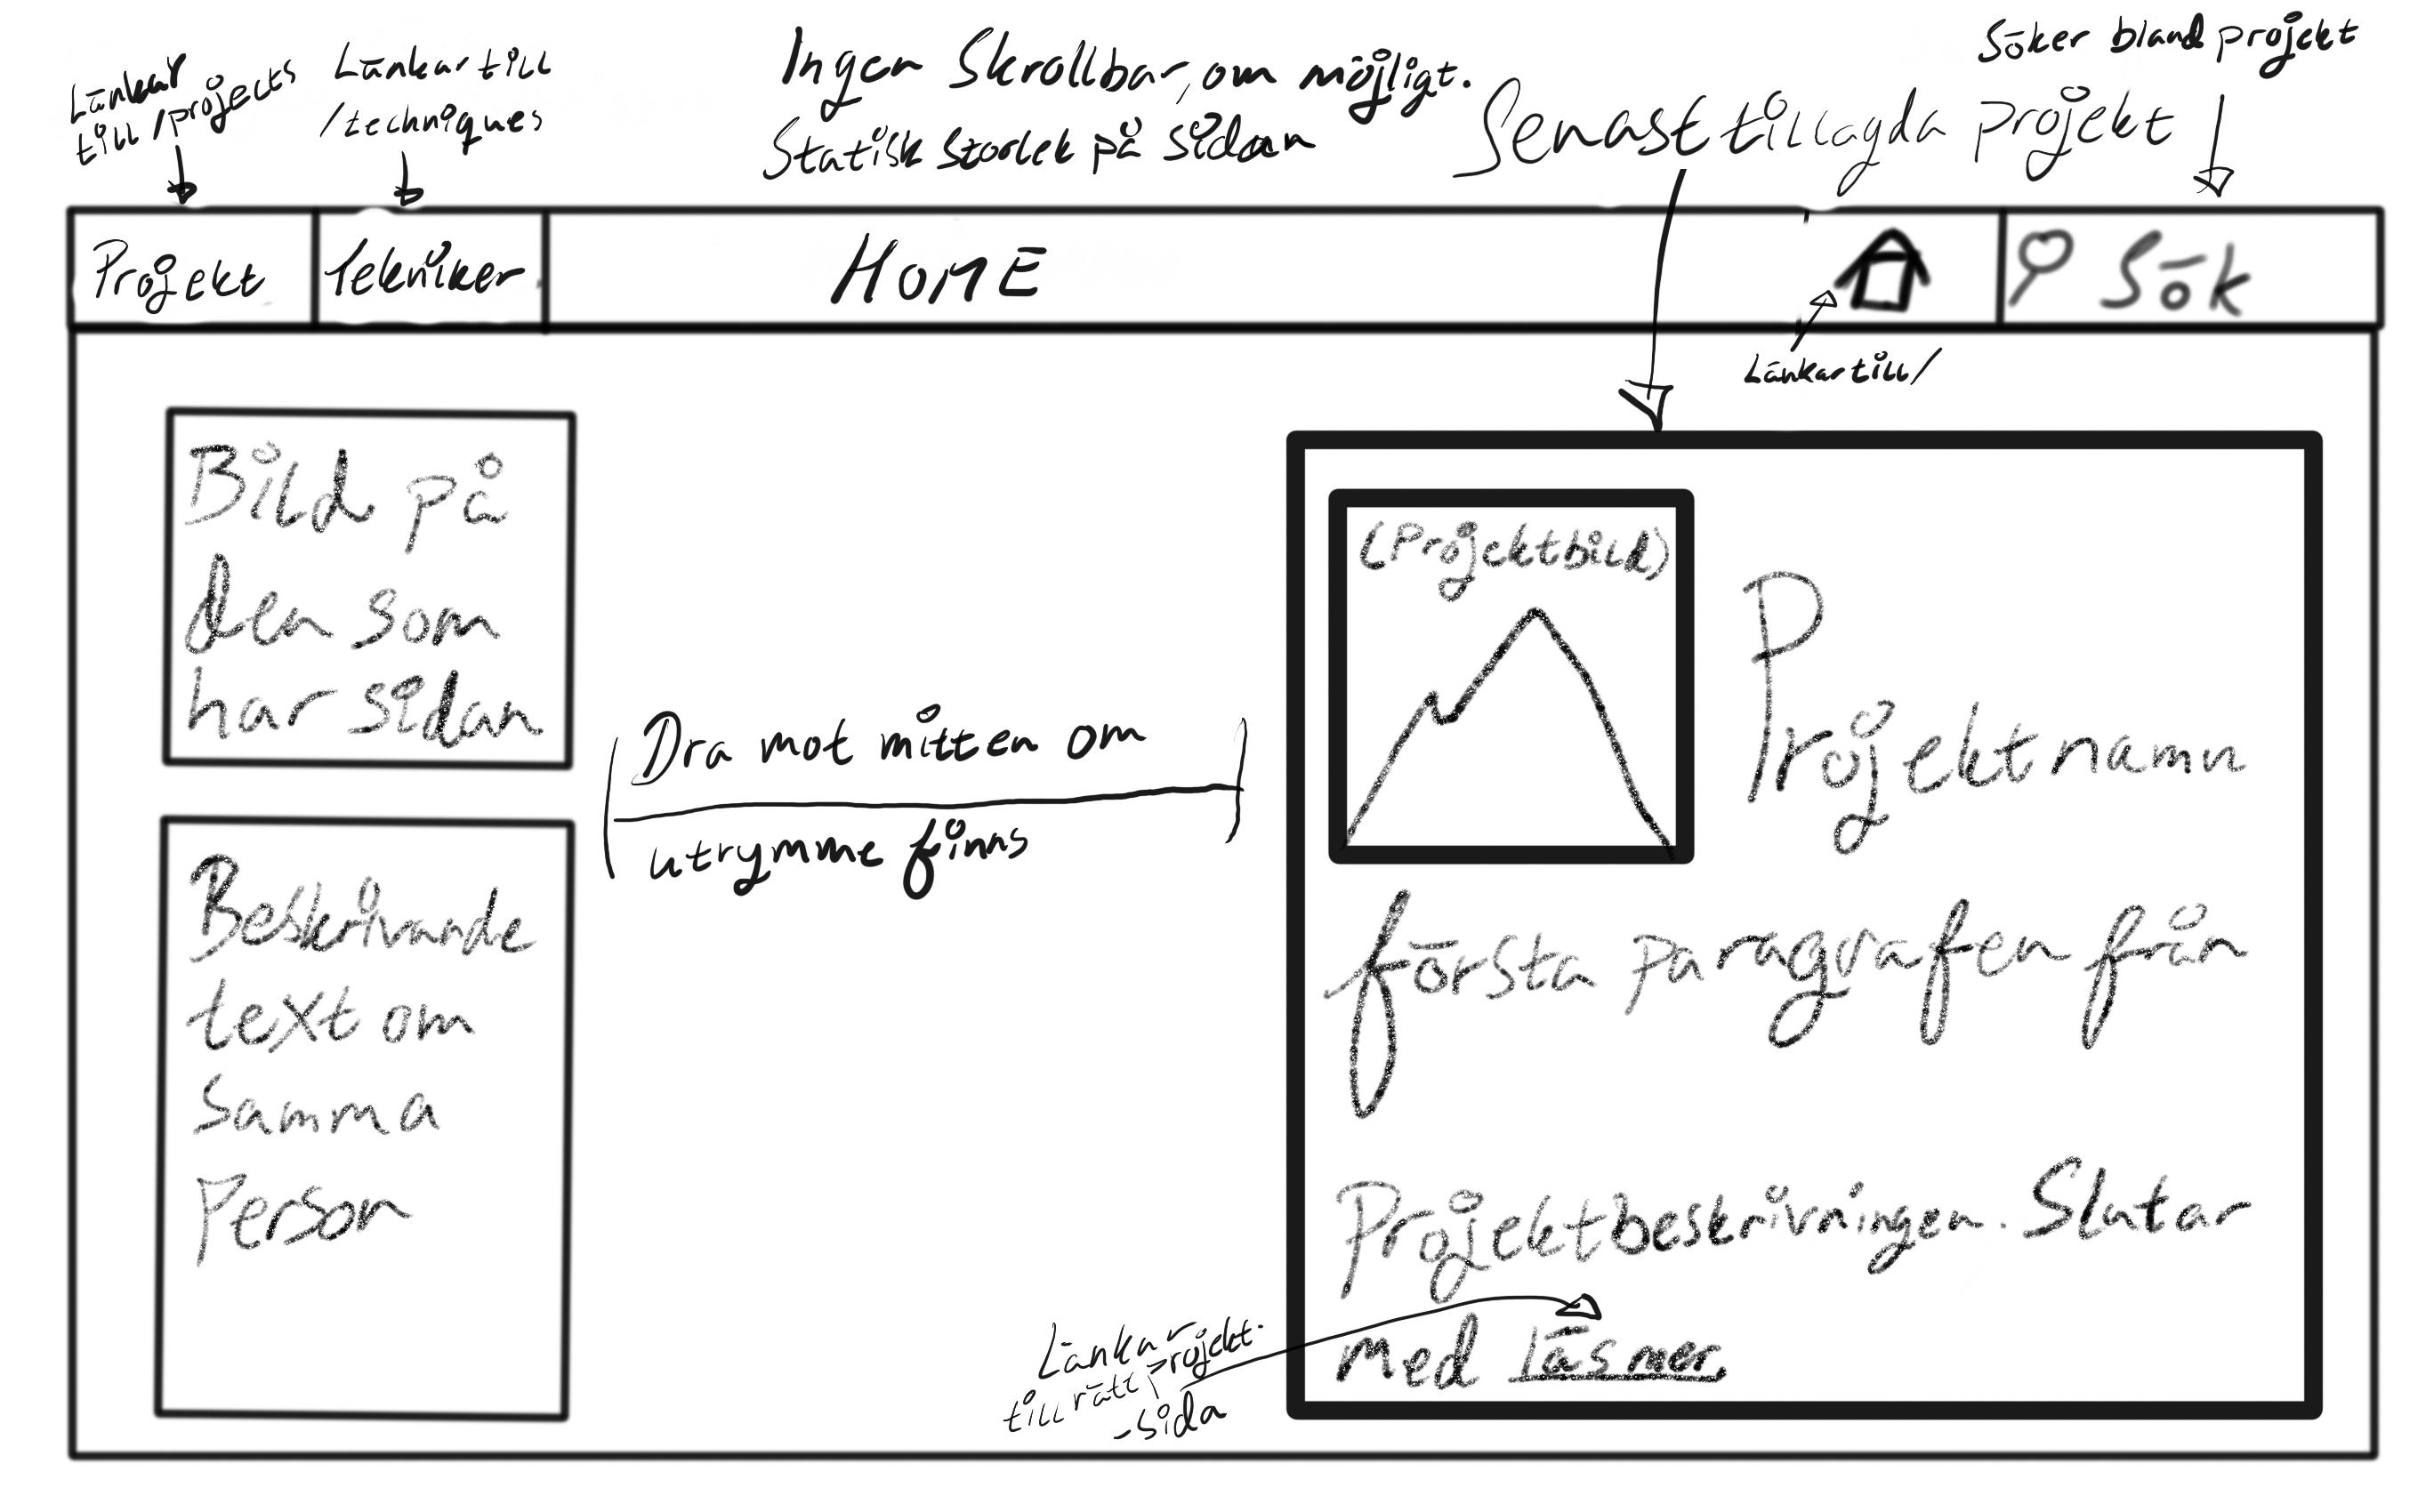
\includegraphics[width=\linewidth]{index.jpg}
  \caption{Skiss på startsidan}
  \label{fig:index}
\end{figure}

\section{Projektlista}
\begin{figure}[H]
  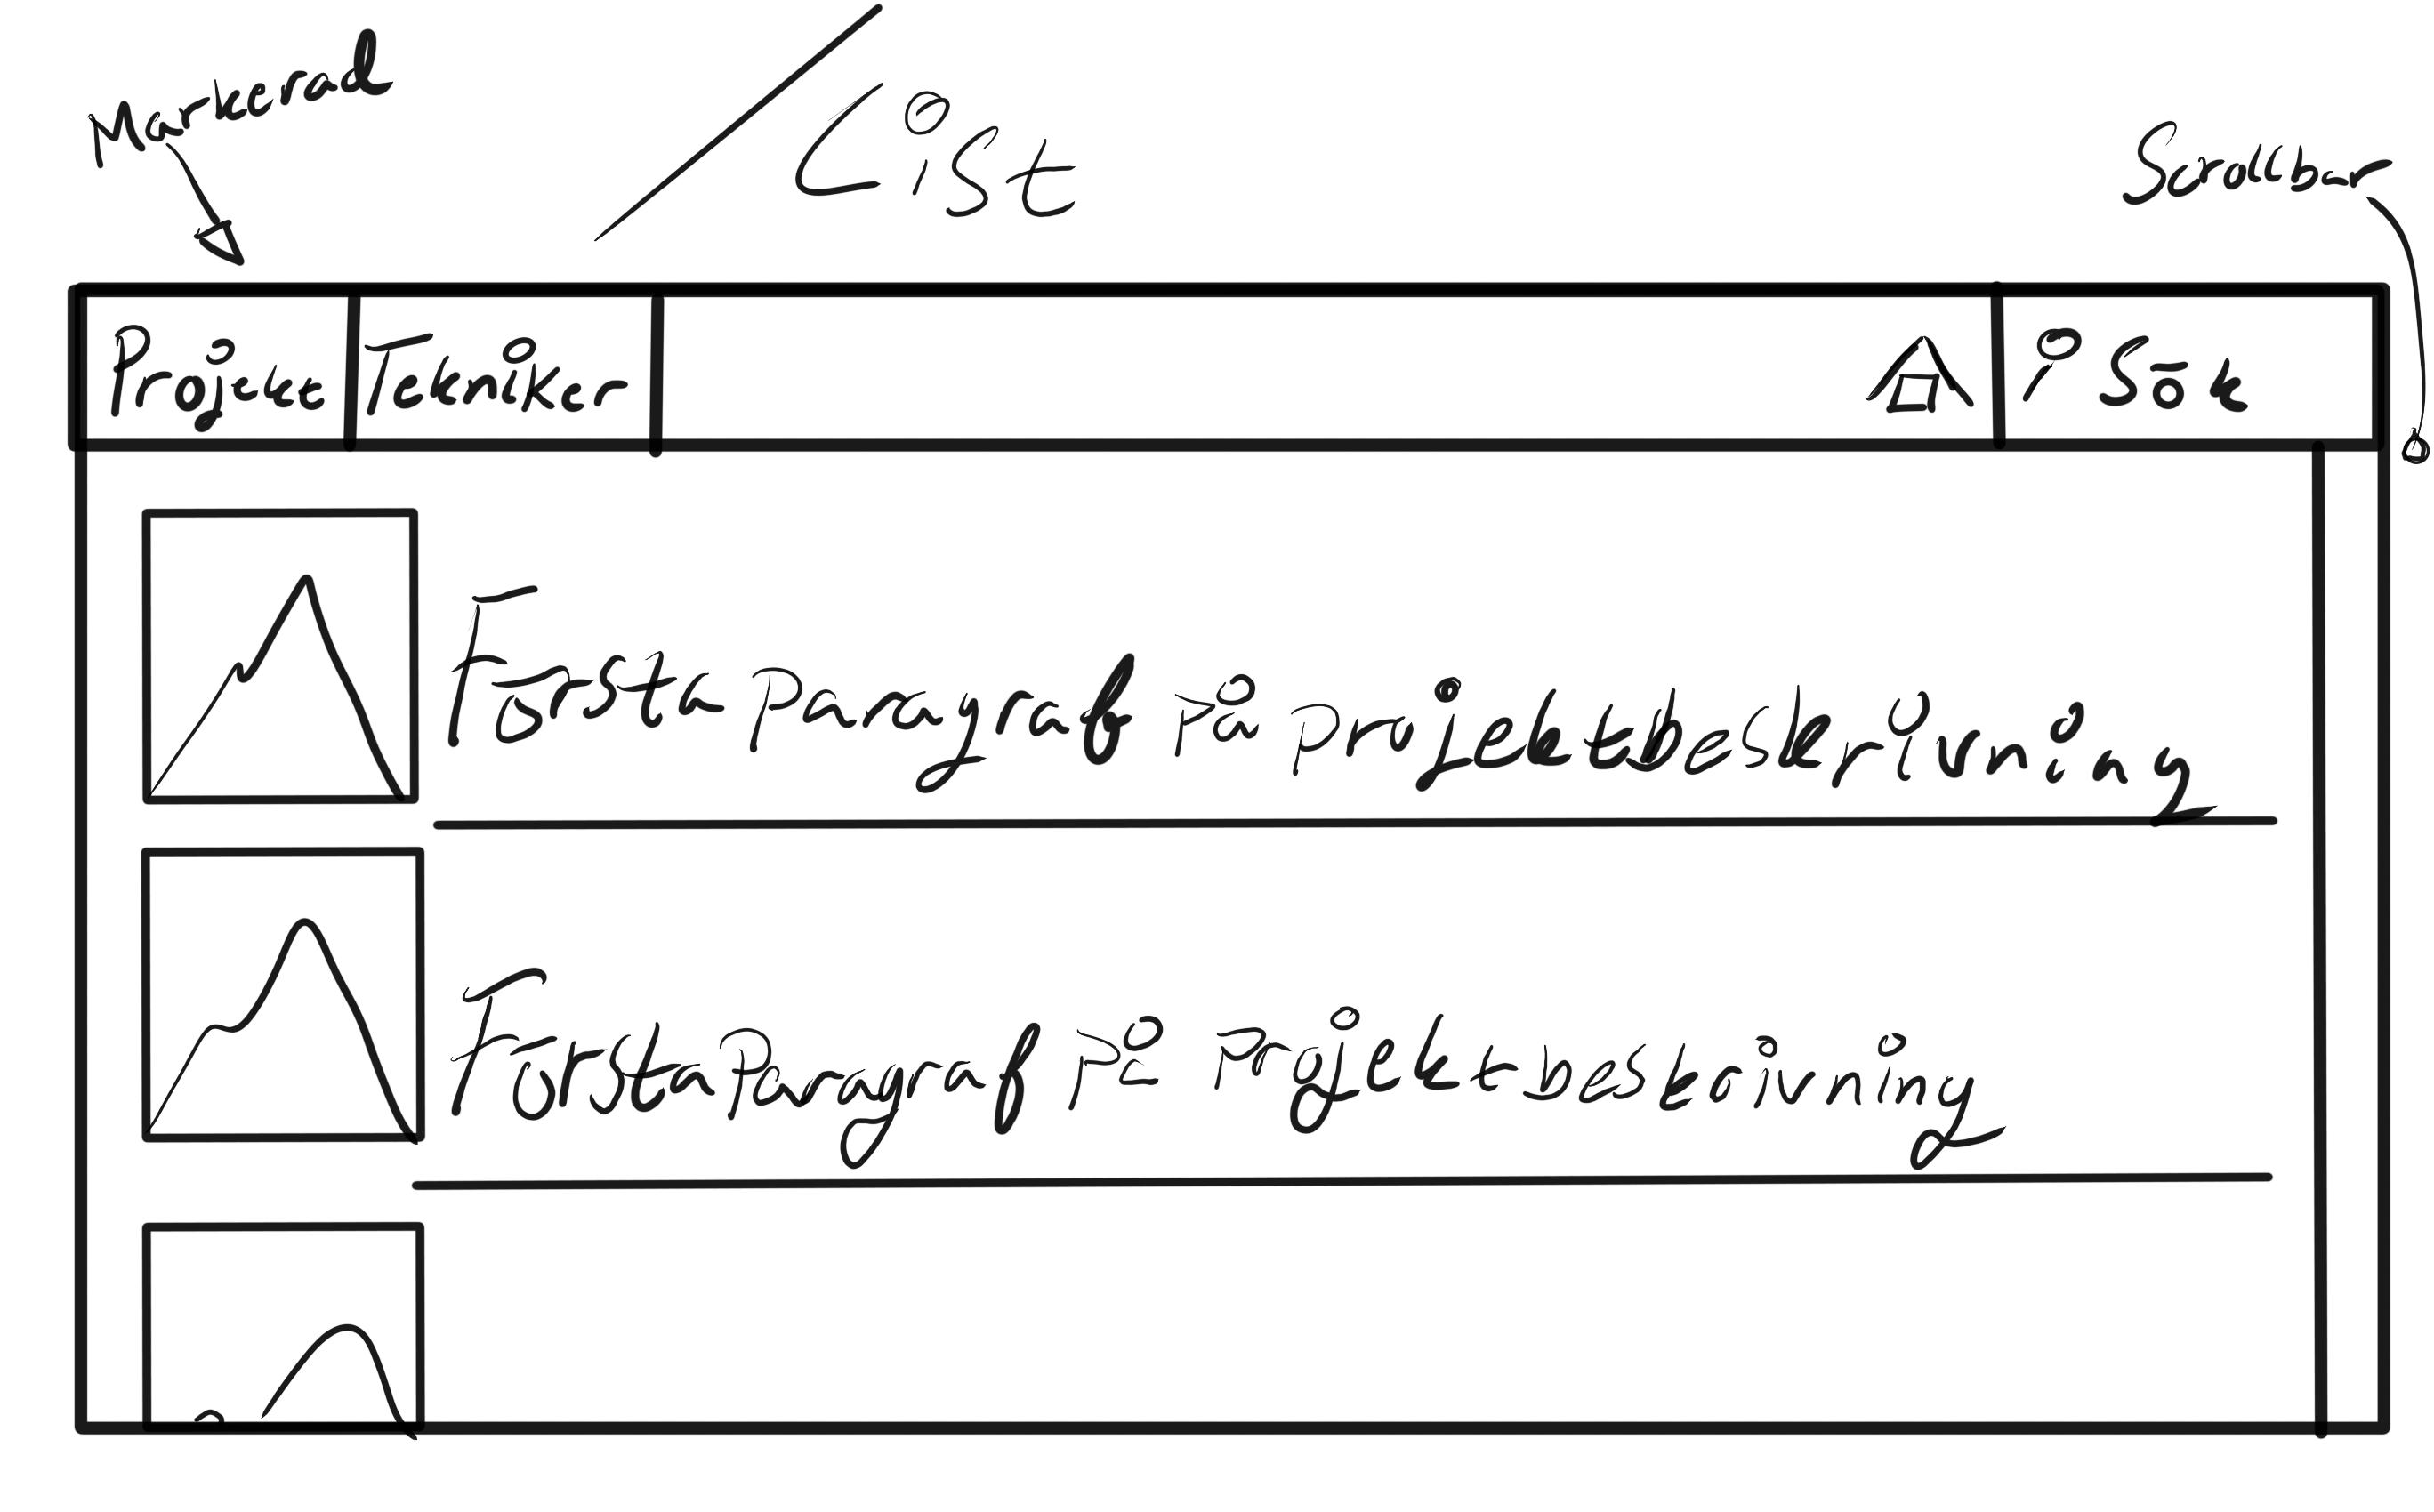
\includegraphics[width=\linewidth]{list.jpg}
  \caption{Skiss på listan av projekt}
  \label{fig:projektlista}
\end{figure}

\section{Tekniksida}
\begin{figure}[H]
  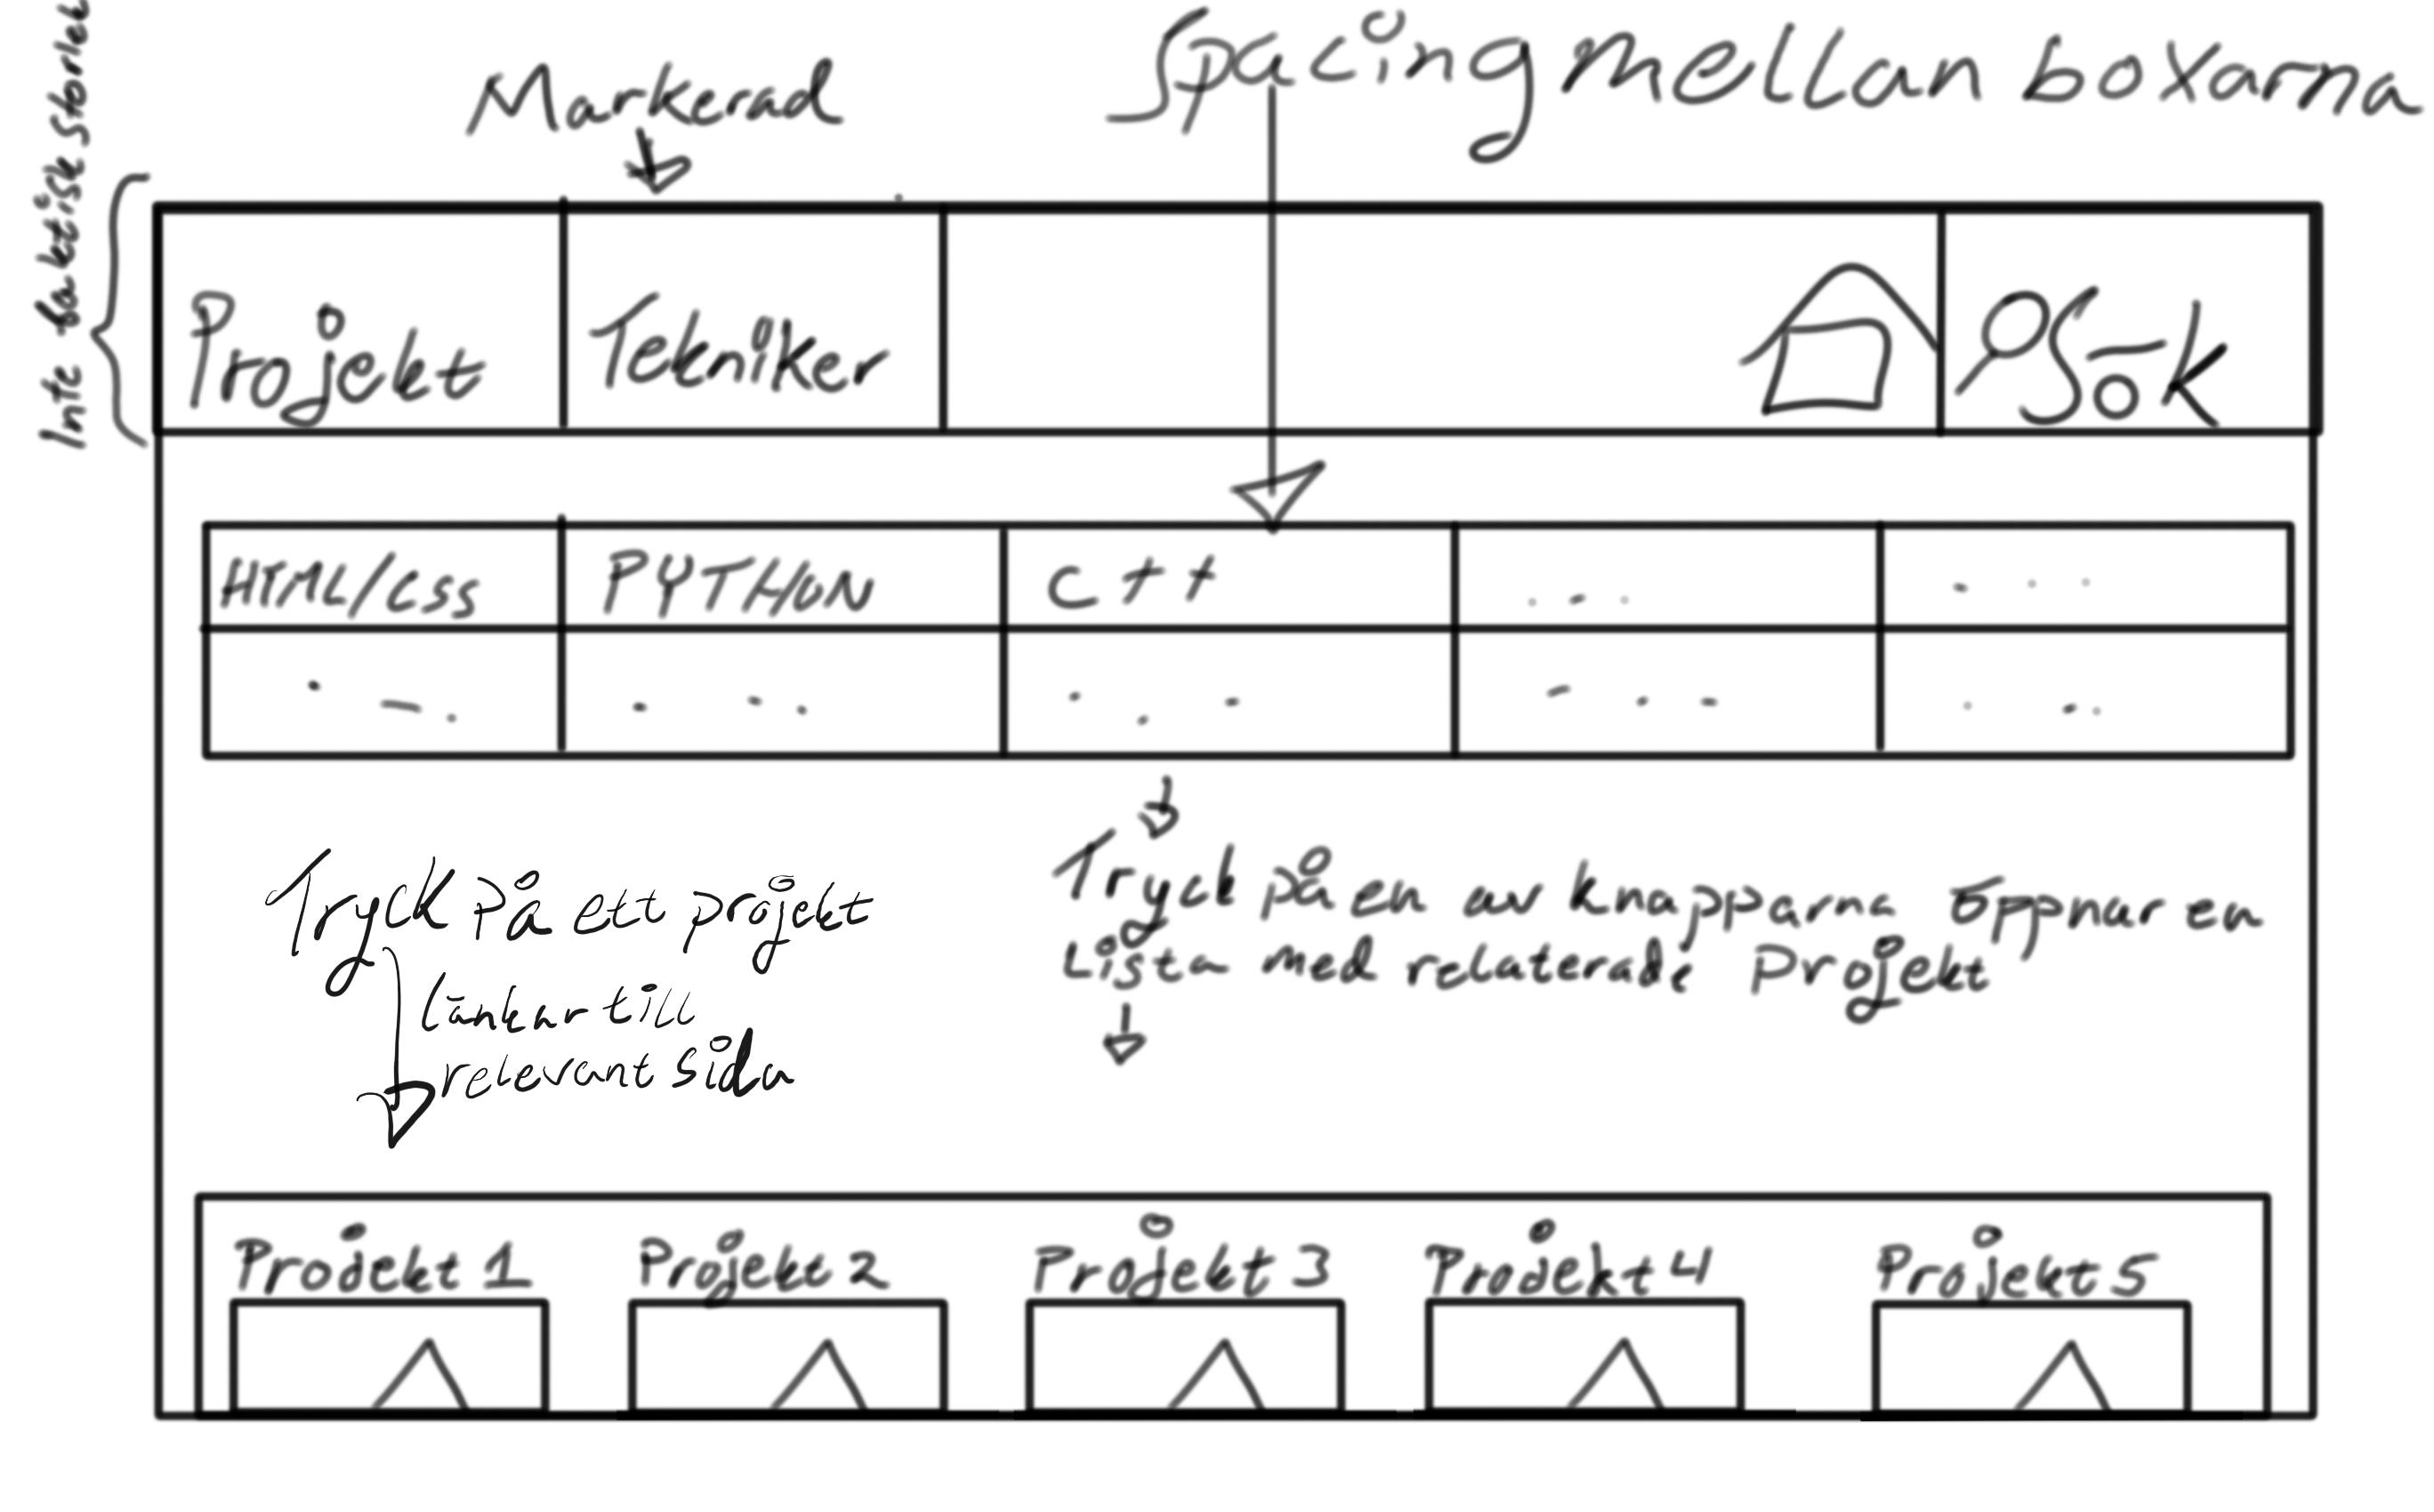
\includegraphics[width=\linewidth]{tekniker.jpg}
  \caption{Skiss på tekniksidan}
  \label{fig:index}
\end{figure}

\section{Projektsida}
\begin{figure}[H]
  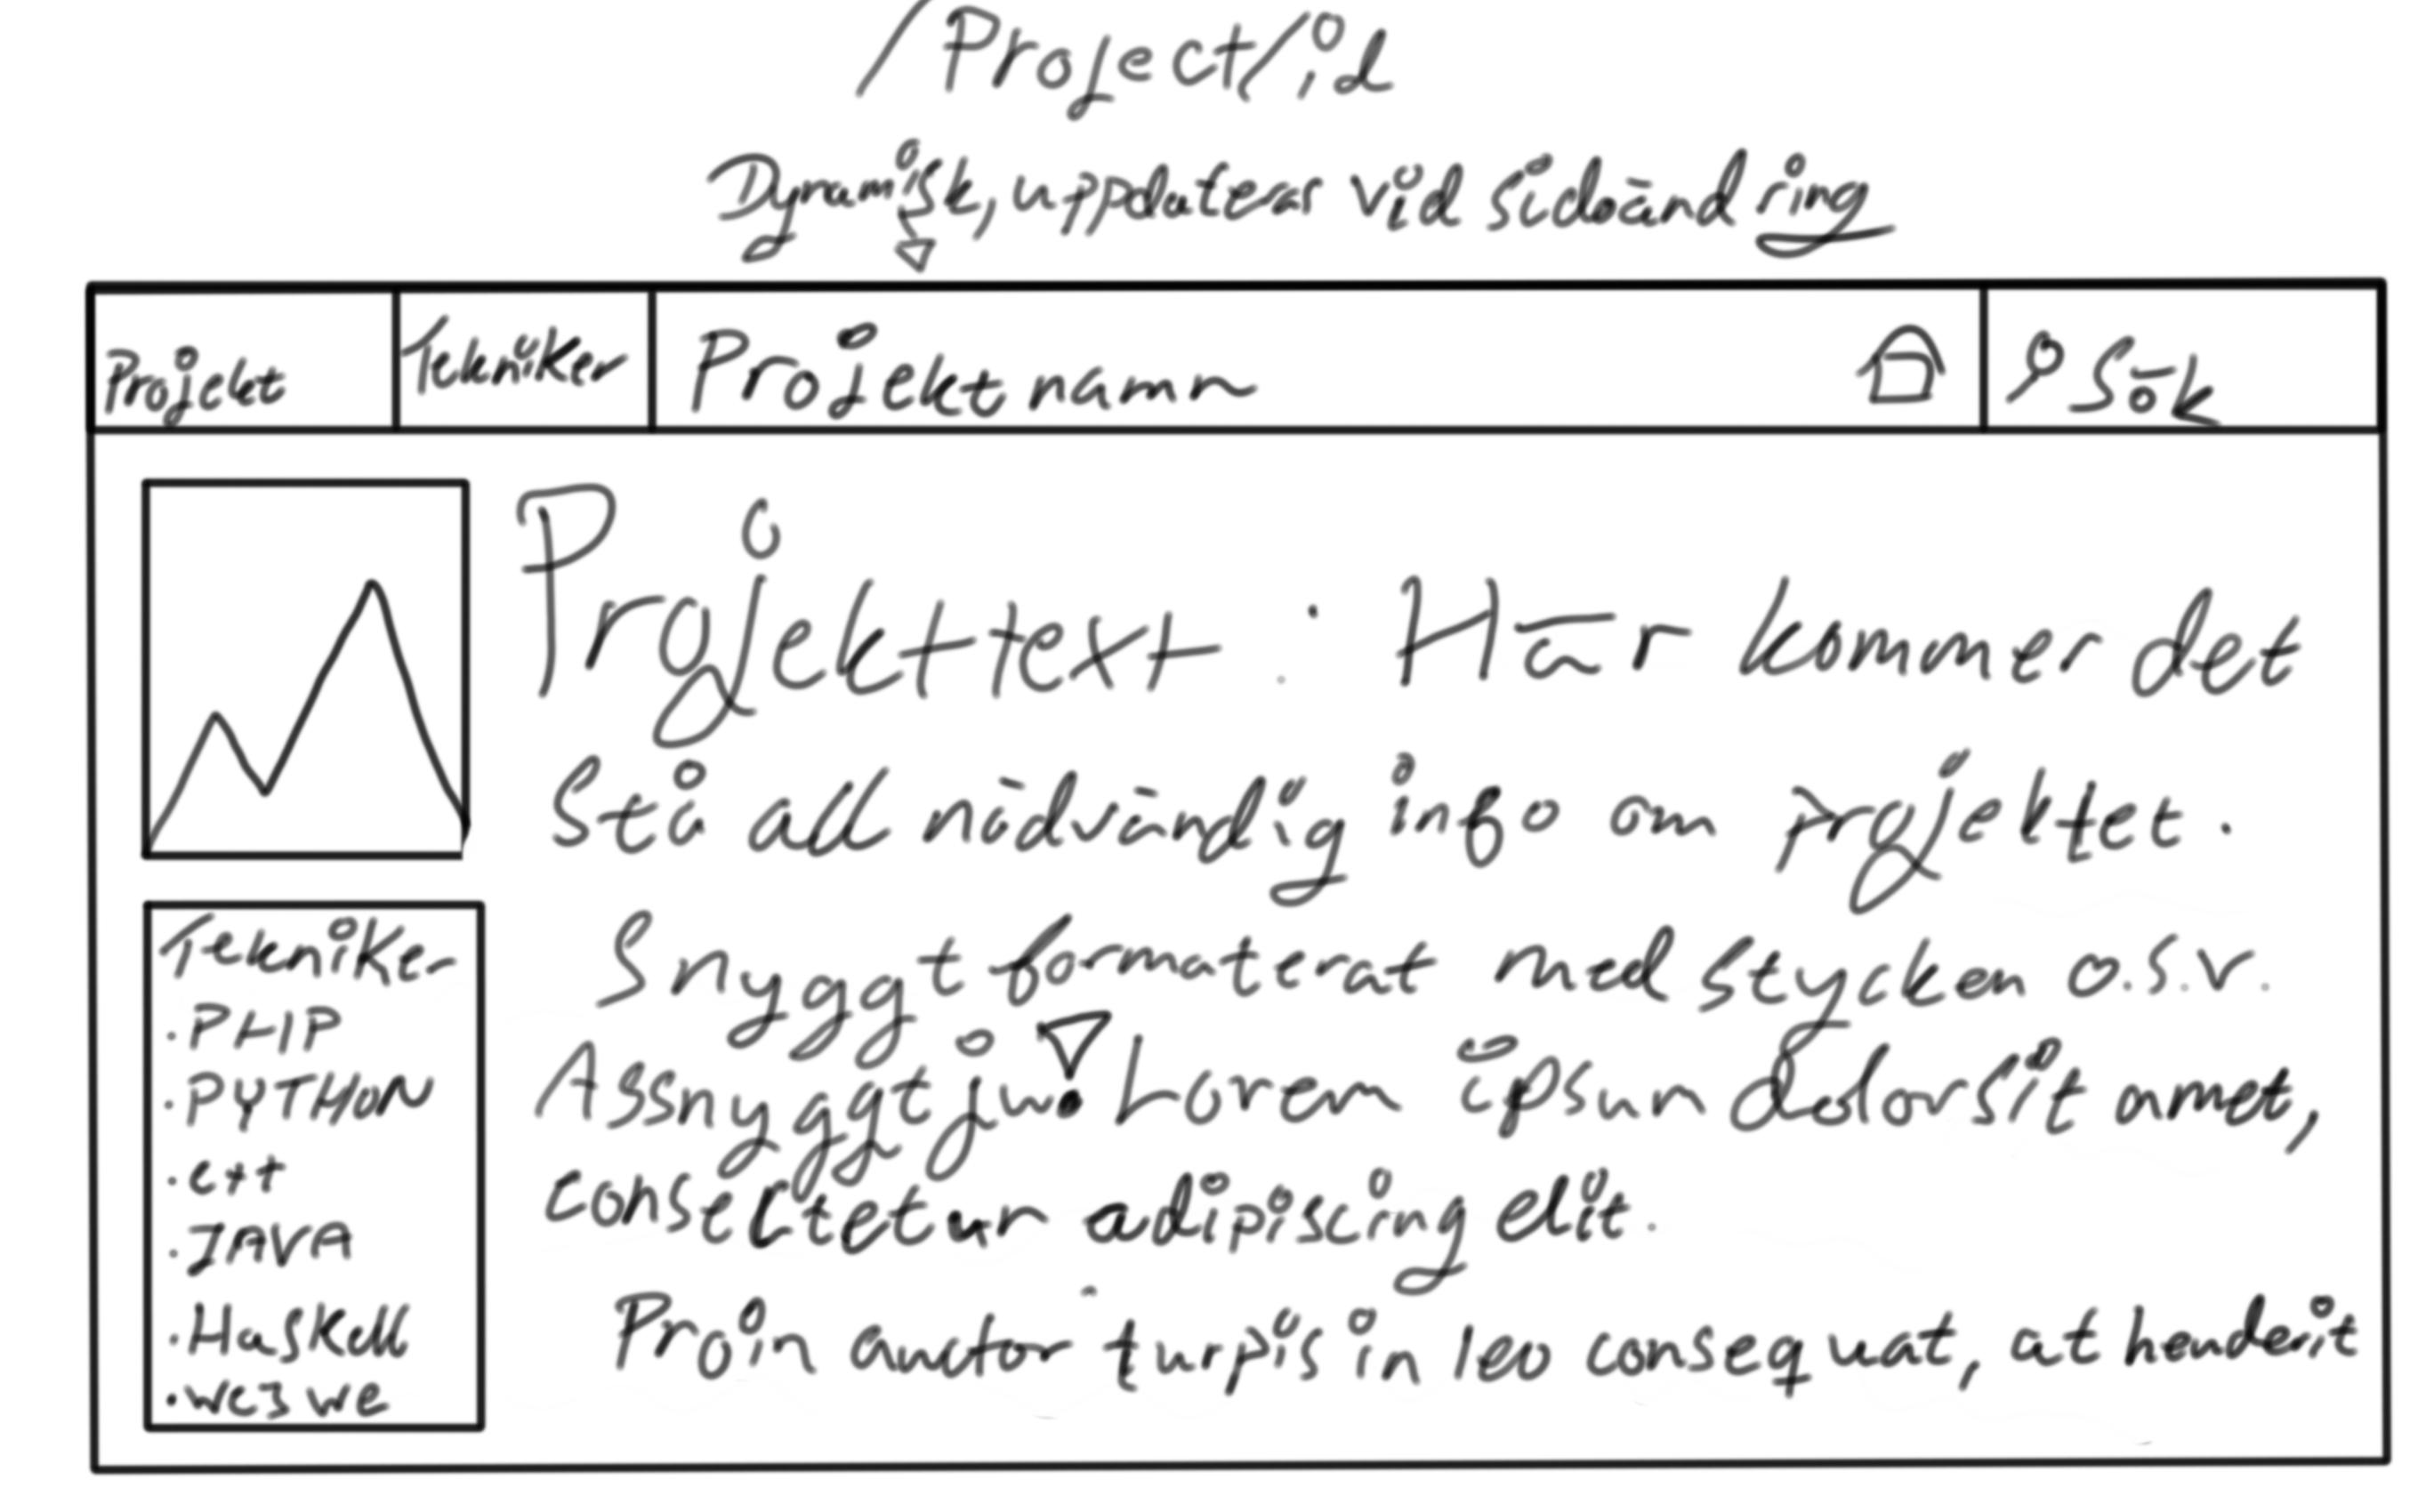
\includegraphics[width=\linewidth]{projekt_id.jpg}
  \caption{Skiss på projektsida}
  \label{fig:index}
\end{figure}

\end{document}
